\documentclass[10pt,conference]{IEEEtran}
\IEEEoverridecommandlockouts
% The preceding line is only needed to identify funding in the first footnote. If that is unneeded, please comment it out.
\usepackage{cite}
\usepackage{amsmath,amssymb,amsfonts}
\usepackage{algorithmic}
\usepackage{graphicx}
\usepackage{textcomp}
\usepackage{booktabs}
\usepackage[table,xcdraw]{xcolor}
\usepackage{framed}
\usepackage{xcolor}
\definecolor{mypink3}{cmyk}{0, 0.7808, 0.4429, 0.1412}

\def\BibTeX{{\rm B\kern-.05em{\sc i\kern-.025em b}\kern-.08em
    T\kern-.1667em\lower.7ex\hbox{E}\kern-.125emX}}

\begin{document}

\title{Security vs. Maintainability: Fixing Vulnerabilities Obfuscates your Code%\\
%\thanks{Identify applicable funding agency here. If none, delete this.}
}

\author{
    Anonymou(s) Author(s)
%     \IEEEauthorblockN{1\textsuperscript{st} Given Name Surname}
% \IEEEauthorblockA{\textit{dept. name of organization (of Aff.)} \\
% \textit{name of organization (of Aff.)}\\
% City, Country \\
% email address}
% \and
% \IEEEauthorblockN{2\textsuperscript{nd} Given Name Surname}
% \IEEEauthorblockA{\textit{dept. name of organization (of Aff.)} \\
% \textit{name of organization (of Aff.)}\\
% City, Country \\
% email address}
% \and
% \IEEEauthorblockN{3\textsuperscript{rd} Given Name Surname}
% \IEEEauthorblockA{\textit{dept. name of organization (of Aff.)} \\
% \textit{name of organization (of Aff.)}\\
% City, Country \\
% email address}
}

\maketitle

\begin{abstract}
  Security is a crucial non-functionality requirement for software applications.
  However, building secure software is far from trivial as developers lack both
  the knowledge and tools to effectively address this concern. In this paper, we
  study the impact of changes to improve security on the maintainability of several
  open source applications. Using a dataset containing XXX security-oriented
  commits, we measure maintainability --- as computed by the Software Improvement
  Group's web-based source code analysis service \emph{Better Code Hub} (BCH) ---
  before and after the security refactoring. Results show that making software
  more secure comes at a cost on  maintainability. This is particularly evident
  in refactorings to deal with \emph{XXX} and \emph{YYY} attacks.
  Furthermore, we have found evidence that security-related changes are more
  likely to be modified in the future than regular code changes.
\end{abstract}

\begin{IEEEkeywords}
Security, Maintainability, Open-Source
\end{IEEEkeywords}

\section{Introduction}

The international standard ISO/IEC 25010:2011 breaks down software quality into eight characteristics: maintainability,
functional suitability, performance efficiency, compatibility, usability, reliability, security,
and portability. This paper focuses solely on maintainability.

\begin{framed}
\textit{\textbf{RQ1} What is the impact of fixing vulnerabilities to improve security }
\end{framed}

\section{Related Work}



\section{Methodology}



\subsection{Dataset}

\begin{table*}[h]
\centering
\caption{Descriptive statistics of the dataset projects\textcolor{mypink3}{@update}} \label{tab:dataset}
\begin{tabular}{@{}ccccccccccc@{}}
\toprule
     & forks   & stars   & watchers & contributors & commits  & branches & releases & size      & issues  & pull requests \\ \midrule
Mean & 1734.79 & 5262.97 & 395.11   & 152.48       & 22257.82 & 44.08    & 126.31   & 143243.64 & 3725.4  & 1976.92       \\
Min     & 1       & 3       & 1        & 0            & 103      & 1        & 0        & 108       & 0       & 0             \\
25 \%     & 374.75  & 1571.5  & 117.75   & 48           & 1347     & 4        & 22       & 8339.5    & 321.25  & 151.75        \\
Median     & 887     & 2836.5  & 258.5    & 102.5        & 5823     & 9        & 59       & 38331.5   & 1652.5  & 515.5         \\
75 \%     & 2196    & 6455.75 & 462.5    & 259          & 22786.25 & 22.25    & 142.25   & 164442.5  & 4152.75 & 1944.25       \\
Max     & 16366   & 31841   & 3446     & 413          & 717449   & 1227     & 1114     & 2042017   & 33970   & 19329         \\
Total     & 180418  & 547349  & 41091    & 15858        & 2314813  & 4584     & 13136    & 14897339  & 387442  & 205600        \\ \bottomrule
\end{tabular}
\end{table*}



\subsection{Security vs. Baseline Commits}



\subsection{Maintainability}


\begin{figure}[h]
 	\centering
 	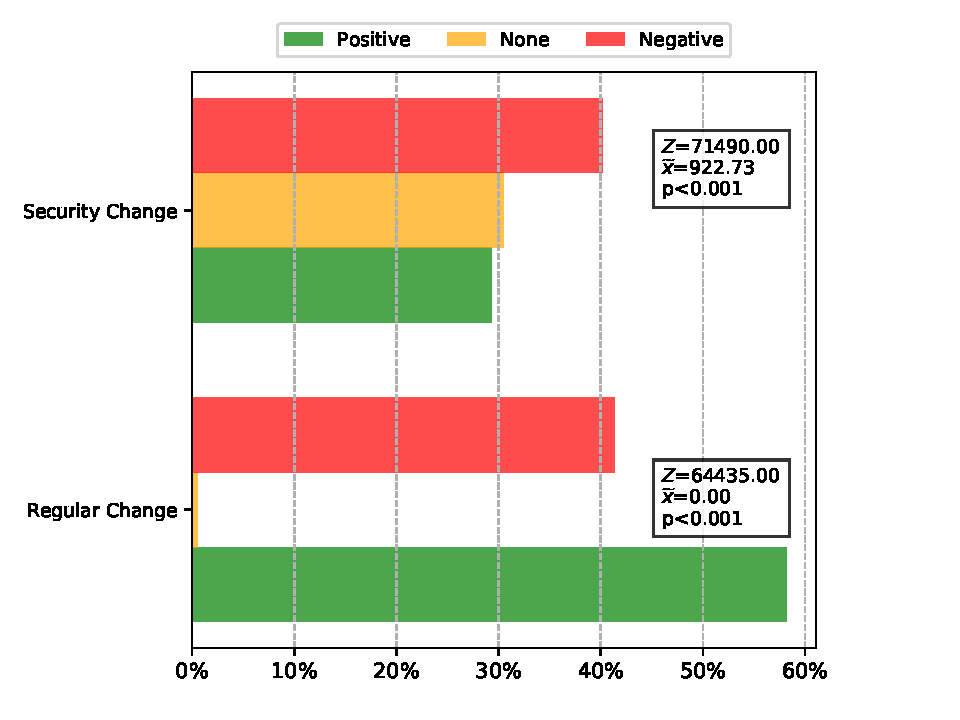
\includegraphics[width=0.4\textwidth]{figures/maintainability.pdf}
 	\caption{Maintainability difference for security and baseline commits \textcolor{mypink3}{@update}}
\end{figure}

\begin{figure}[h]
 	\centering
 	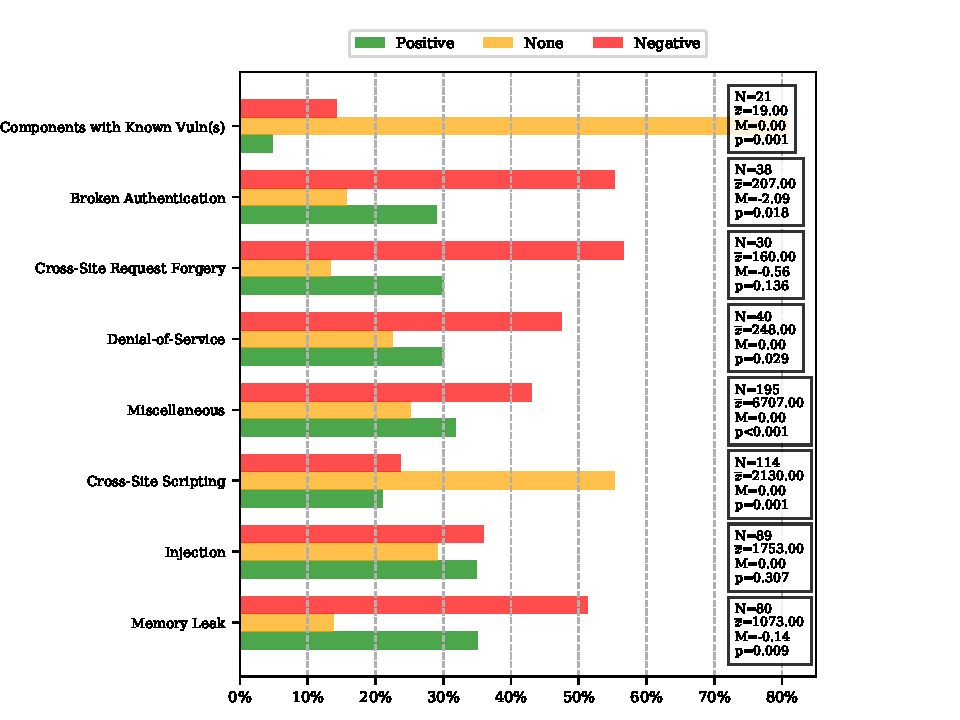
\includegraphics[width=0.55\textwidth]{figures/category.pdf}
 	\caption{Maintainability difference by type of security commit \textcolor{mypink3}{@update}}
\end{figure}


\cite{Wang:2008:DSJ:1330017.1330021}


\section{Results}




\section{Discussion}


\section{Threats to Validity}


\section{Conclusion}



\section*{Acknowledgment}

{
 \bibliographystyle{IEEEtran}
  \bibliography{icpc19}
}

\end{document}
